\documentclass[letterpaper,10pt,conference]{ieeeconf}
\usepackage[T1]{fontenc}
\let\proof\relax
\let\endproof\relax
\usepackage{amsmath,amssymb,amsthm,booktabs,graphicx,array}
\usepackage{xcolor}
\usepackage[hidelinks]{hyperref}
\newtheorem{proposition}{Proposition}
\newcommand{\E}{\mathbb{E}}
\newcommand{\PDMS}{\mathrm{PDMS}}
\newcommand{\NC}{\mathrm{NC}}
\newcommand{\DAC}{\mathrm{DAC}}
\newcommand{\TTC}{\mathrm{TTC}}
\title{Beyond Safety Filtering: How Training Targets Shape Driving Policy Improvement}
\author{\phantom{Anonymous Authors}}

\begin{document}
\raggedbottom
\maketitle
\begin{abstract}
High-scoring trajectories that pass safety checks are natural post-training targets, but candidate quality need not predict training usefulness. We study winner selection in a frozen-backbone flow-matching driving policy, holding candidates, safety gates, losers, and fitting fixed. On all NAVSIM navtest scenes under v1 scoring, all four score-winner runs introduce more failures than they repair in each of three safety components, whereas all eight geometric-winner runs show the opposite balance. At every matched seed, geometric rules exceed score selection in total and safety-component scores, with paired 95\% log-cluster intervals above zero. Random eligible winners also outperform score selection at three matched seeds: their mean advantage is 0.96 points [0.63,1.30]. Total-score differences from geometric rules remain unresolved, although geometry retains safety-component advantages. We derive winner-dependent updates and a conditional feasibility bound, and distinguish repaired failures from lost successes. Geometric-versus-score advantages persist in four-seed v2 re-scoring under non-reactive and reactive traffic, but gains over the supervised baseline remain unresolved and lane keeping declines. The results motivate evaluating supervision through downstream repair and preservation, including behavior beyond the target-verification gates.
\end{abstract}


\section{Introduction}
A driving policy can generate several trajectories that pass a simulator's safety checks. Using these candidates for post-training requires a second decision: which passing trajectory should the policy learn from? Choosing the highest-scoring candidate seems natural. It has passed verification and optimizes the same quantity used to evaluate the policy. Yet its score describes one trajectory in one scene, whereas fitting that trajectory changes a policy shared across many scenes.

This distinction matters when the reference policy already succeeds on most inputs. An update may repair a difficult case while introducing failures elsewhere, and an aggregate score can offset those failures with greater progress. Evaluating the selected target alone cannot reveal this balance. The relevant question is therefore not only whether a candidate is acceptable, but whether preferring it produces a policy that repairs more than it breaks.

Preference-data studies have established that the choice of training examples affects learning~\cite{sweetspot,whatmatters,correctanswers}. In driving, however, candidate acceptance and target selection are often closely coupled: simulator checks define eligible trajectories, and a score or geometric rule selects the preferred \emph{winner} over a rejected \emph{loser}. We examine the choice left after verification: \emph{among the same passing candidates, does the highest-scoring winner produce the strongest policy?} Using DriveVLA-W0~\cite{drivevla}, we hold candidates, safety gates, loser construction, and fitting fixed. Winners maximize driving score, maximize obstacle clearance, or minimize reference displacement. 

\textbf{Higher-scoring verified targets need not yield better policies.} On full navtest under v1 evaluation, all four score-winner policies introduce more failures than they repair in each safety component, while all eight geometric-winner policies show the reverse (Fig.~\ref{fig:framework}). Both geometric rules exceed score selection at every matched seed, with lower progress than the score-trained policy. Their gains over supervised fine-tuning (SFT) range from 0.40 to 1.02 PDMS points. Crucially, uniformly selected eligible winners also exceed score selection at three matched seeds. Their aggregate-score differences from the geometric rules remain unresolved, while geometry retains safety-component advantages. The comparison therefore questions the highest-score target as a default, rather than establishing geometry as necessary for improvement.

\textbf{Improvement within the original gates is not comprehensive preservation.} The geometric-versus-score advantage persists in four-seed v2 comparisons under non-reactive and reactive traffic. Yet no tested rule has a resolved v2 total-score gain over SFT, and all lose lane-keeping performance. These outcomes motivate evaluating both failures repaired and successes lost, including behaviors not directly checked when selecting targets.

Our analysis connects winner choice to the fitting gradient and states conditions under which target feasibility transfers to the fitted policy. A repair--regression ledger separates recovered failures from lost successes, and privileged candidate ranking on two DriveVLA-W0 variants shows how much opportunity the candidate pool contains.

We make three contributions to understanding verified post-training:
\begin{itemize}
\item  With safety eligibility and fitting fixed, winner choice reverses the repair balance across twelve primary runs. A three-seed random-eligible control shows that improvement over score-maximizing targets does not require explicit geometric ranking.
\item We derive how winner choice enters the shared update and state margin--approximation conditions for feasibility transfer. Target and fitting-error measurements constrain simple explanations without claiming an identified mechanism.
\item  Component-wise repair--regression accounting distinguishes recovered failures from lost successes. V2 re-scoring shows that a favorable comparison within the original safety gates can coexist with deterioration in other behavior.
\end{itemize}

\begin{figure*}[!t]
\centering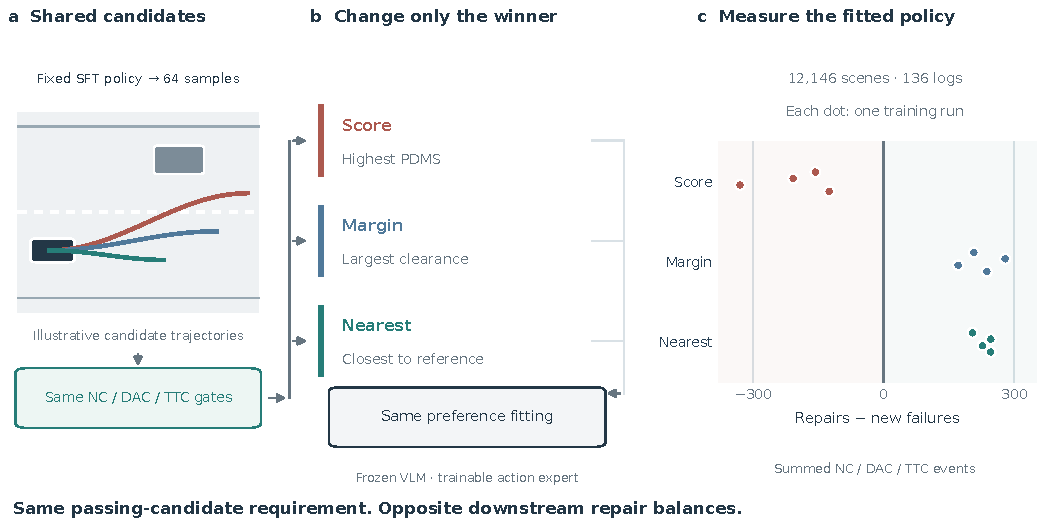
\includegraphics[width=0.8\textwidth]{figures/ral/fig1_framework.pdf}
\caption{\textbf{The same safety filter can lead to opposite repair balances.} (a) A fixed SFT policy supplies candidates checked by the same NC/DAC/TTC gates. The road drawing is illustrative. (b) Only the passing-winner rule changes; loser construction and preference fitting are shared. (c) Measured downstream outcomes on full navtest. Each point is one of the twelve primary runs (the random-winner extension is reported separately); the horizontal axis sums repairs minus new failures over NC, DAC, and TTC, not unique scenes. Matched comparisons appear in Fig.~\ref{fig:target_contrasts}.}
\label{fig:framework}
\end{figure*}

\section{Related Work}
\paragraph{Generative driving policies and post-training}
Diffusion Policy~\cite{diffpolicy} and $\pi_0$~\cite{pi0} model robot actions with diffusion and flow matching, respectively. For driving, DiffusionDrive uses anchored truncated diffusion~\cite{diffdrive}, while DriveVLA-W0 couples world modeling with policy learning~\cite{drivevla}. DiffusionDriveV2 applies intra- and inter-anchor GRPO to improve trajectory quality while preserving diverse intentions~\cite{diffdrivev2}; TakeAD combines expert takeover data with imitation and preference optimization~\cite{takead}. We fix the architecture and fitting recipe to isolate a different decision: which passing candidate should supervise the policy. Our findings do not imply that reinforcement-learning post-training generally fails.

\paragraph{Preference objectives and target construction}
DPO fits pairwise preferences through a reference-relative likelihood objective~\cite{dpo}; diffusion DPO adapts preference optimization to diffusion models~\cite{diffdpo}. Advantage-weighted regression~\cite{awr}, best-of-$N$ distillation~\cite{bond}, and DPPO~\cite{dppo} provide alternative regression, distillation, and policy-gradient routes. We use a fixed flow-loss surrogate~\cite{flowmatching,diffdpo}, not an exact trajectory likelihood ratio. Data construction remains a separate choice: Xiao et al.~\cite{sweetspot} study rejected-response selection, Pan et al.~\cite{whatmatters} examine chosen-response quality, and Tian et al.~\cite{correctanswers} report different student outcomes from verified teacher traces. Our comparison fixes candidate source and loser construction and tests winner choice within one passing set.

\paragraph{Geometric preferences and safety constraints}
DriveReferee constructs geometric preferences and compares maximum-margin with nearest-expert winners~\cite{drivereferee}. We include a score-maximizing winner under identical simulator gates, use a reference prediction rather than the expert as the nearest anchor, and measure downstream repairs and regressions. Constrained Policy Optimization constrains expected costs during policy updates~\cite{cpo}; shielding restricts or corrects actions using a safety specification~\cite{shielding}. Our filter instead qualifies stored training targets. It neither constrains all outputs of the fitted policy nor provides a runtime shield. The conditional feasibility analysis makes this distinction explicit.

\paragraph{Transfer and driving evaluation}
DAgger addresses the state-distribution shift induced by learned actions through interactive data aggregation~\cite{dagger}. Our fixed-scene approximation analysis does not address that closed-loop shift. NAVSIM supplies non-reactive planning evaluation~\cite{navsim}, while its v2 pseudo-simulation protocol extends evaluation beyond a single logged scene~\cite{navsimv2}. We distinguish v1 results from one-stage v2 re-scoring and count preserved successes alongside repaired failures; neither evaluation establishes closed-loop policy safety.

\section{Verified Targets and Policy Improvement}
Our study separates three decisions: which candidates pass verification, which passing candidate becomes supervision, and how fitting that target changes the policy. The analysis follows the same sequence: it identifies the winner-dependent update, the preference retained after filtering, and the conditions needed to preserve feasibility after approximation.
\subsection{Controlled target construction}
Let $s$ denote a scene, $o(s)$ its policy observation, and $\mathcal A_s$ a pool of trajectories sampled from reference policy $\pi_0$. Using no-at-fault collision (NC), drivable-area compliance (DAC), and time-to-collision (TTC) checks, define the eligible set
\begin{equation}
\mathcal E_s=\{a\in\mathcal A_s:\NC(s,a)=\DAC(s,a)=\TTC(s,a)=1\}.
\end{equation}
For scenes with both eligible and ineligible candidates, we choose a winner by one of three rules:
\begin{align}
a^+_{\rm score}&=\arg\max_{a\in\mathcal E_s}\PDMS(s,a),\nonumber\\
a^+_{\rm margin}&=\arg\max_{a\in\mathcal E_s}m(s,a),\label{eq:rules}\\
a^+_{\rm near}&=\arg\min_{a\in\mathcal E_s}d(a,a_0(s)).\nonumber
\end{align}
We define obstacle clearance as the signed gap between the approximate ego and surrounding-agent footprints: positive values indicate separation, and negative values indicate overlap. Footprints are approximated by covering circles, and surrounding agents are predicted under constant velocity from their time-zero states. The selection margin $m(s,a)$ is the minimum clearance over all surrounding agents and the eight future waypoints. This geometric quantity is distinct from the simulator's NC, DAC, and TTC checks.

The nearest rule uses mean planar waypoint distance to $a_0$, the pointwise mean of the stored reference-probe trajectories. This reference is a target-selection anchor, not the expert demonstration. Ties retain the first candidate in the stored ordering.

The loser is the ineligible candidate nearest the expert trajectory in normalized action space. Relative $(x,y,\mathrm{heading})$ increments are affinely normalized with the stored 1st/99th-percentile bounds, without clipping; distance is Euclidean over the flattened trajectory. Scenes without a mixed pair are omitted. Thus the three standard rules use the same scene-eligibility criterion, qualifying set, and loser construction. Geometry enters target construction during training, while the fitted policy retains its original observation interface at inference.

Let $a^E$ denote the expert trajectory, $\ell_\theta(a;s,\xi)$ the flow-matching squared error for noise/time draw $\xi$, and $\ell_0(a;s,\xi)$ the corresponding loss of the frozen reference policy. We use
\begin{align}
d_\theta&=[\ell_\theta(a^+)-\ell_0(a^+)]-[\ell_\theta(a^-)-\ell_0(a^-)],\nonumber\\
\mathcal L&=\operatorname{softplus}(\beta d_\theta)+\lambda_w\ell_\theta(a^+)
 +\lambda_E\ell_\theta(a^E).\label{eq:pref}
\end{align}
The winner-fitting term $\lambda_w\ell_\theta(a^+)$ is a separate supervised objective, combined with the pairwise preference loss. The expert-anchor term is applied at the update level. The backbone stays frozen; only the action expert is fitted. This is a flow-loss surrogate, not an exact trajectory likelihood ratio. All target rules use the same training setting.

\subsection{How the winner changes the update}
Write $g^+_w=\nabla_\theta\ell_\theta(a^+_w)$, $g^-=\nabla_\theta\ell_\theta(a^-)$, and $g^E=\nabla_\theta\ell_\theta(a^E)$ for one matched loss evaluation. With the reference detached and $\sigma$ the logistic function, differentiating Eq.~\eqref{eq:pref} gives
\begin{equation}
\nabla_\theta\mathcal L_w
=(\beta\sigma(\beta d_w)+\lambda_w)g^+_w
-\beta\sigma(\beta d_w)g^-+\lambda_E g^E.
\label{eq:gradient}
\end{equation}
The winner affects both its own fitting gradient and, through $d_w$, the coefficient of the loser gradient. Keeping the loser fixed therefore does not make the preference update independent of winner choice.

\begin{proposition}[Winner dependence at initialization]\label{prop:update}
Suppose the fitted and reference policies coincide at initialization, their losses use matched noise/time draws, and two winner rules share the scene, loser, and expert anchor. Their initial loss-gradient difference is
\begin{equation}
\nabla\mathcal L_u-\nabla\mathcal L_v
=(\beta/2+\lambda_w)(g^+_u-g^+_v).
\label{eq:gradientdiff}
\end{equation}
The same statement holds after averaging matched loss evaluations.
\end{proposition}
\begin{proof}
At initialization, each current-minus-reference loss is zero, hence $d_u=d_v=0$ and $\sigma(0)=1/2$. Subtracting Eq.~\eqref{eq:gradient} cancels the common loser and expert terms.
\end{proof}
The shared expert anchor therefore does not cancel the initial winner-dependent gradient. This local result neither models the full Adam trajectory nor predicts the sign of downstream safety changes; those are measured by the matched policy evaluations.

\subsection{What remains after safety filtering?}
\label{sec:ordering}

Safety filtering fixes $\mathcal E_s$, not the target distribution $Q_w(\cdot\mid s)$ induced by rule $w$. The shared objective becomes
\begin{equation}
\mathcal J_w(\theta\mid s)=\E_{A^+\sim Q_w,\,\xi}[\mathcal L_\theta(A^+,a^-;s,\xi)].
\label{eq:target_objective}
\end{equation}
For deterministic rules, $Q_w$ is a point mass at the winner. Among passing candidates with equal comfort, maximizing PDMS is equivalent to maximizing evaluated progress; margin and nearest instead favor clearance and reference proximity. These preferences change supervision despite identical acceptance criteria. Progress measures route advancement, not simply speed.

\subsection{From target quality to policy behavior}
A verified target and a fitted-policy output need not coincide. Let $P_w(\cdot\mid s)$ denote the policy fitted using winner rule $w$, and $\mathcal D$ a common scene distribution. For a bounded utility $f$, define $J_f(P)=\E_{s\sim\mathcal D,\,a\sim P(\cdot\mid s)}[f(s,a)]$. The identity
\begin{equation}
\begin{split}
J_f(P_w)-J_f(\pi_0)
={}&J_f(Q_w)-J_f(\pi_0)\\
&-[J_f(Q_w)-J_f(P_w)]
\end{split}
\label{eq:transfer}
\end{equation}
separates target improvement from a signed transfer discrepancy. Maximizing the former need not maximize policy performance because the latter also depends on the winner rule. This is an accounting identity, not a mechanism estimate. In particular, subtracting our privileged-ranking and policy-fitting gains would not estimate this discrepancy: their information and inference budgets differ.

\subsection{Feasibility under target approximation}
Let $c_s(a)$ be a signed constraint margin, positive for feasible trajectories, and assume $|c_s(a)-c_s(a')|\leq L\|a-a'\|$ for a fixed trajectory norm and uniform $L>0$. Couple a target $A^+\sim Q_w(\cdot\mid s)$ and fitted output $\widehat A\sim P_w(\cdot\mid s)$ on the same scene distribution, and define
\begin{equation}
\epsilon_w^2=\E\|\widehat A-A^+\|^2.
\label{eq:transfer_error}
\end{equation}
The coupling specifies how targets and outputs are paired and must have finite second moment.

\begin{proposition}[Feasibility under target approximation]\label{prop:margin}
For every $\gamma>0$,
\begin{equation}
\Pr[c_s(\widehat A)\leq0]
\leq\Pr[c_s(A^+)\leq\gamma]+\frac{L^2\epsilon_w^2}{\gamma^2}.
\label{eq:marginerror}
\end{equation}
\end{proposition}
\begin{proof}
If $c_s(A^+)>\gamma$ and $\|\widehat A-A^+\|<\gamma/L$, Lipschitz continuity gives $c_s(\widehat A)>0$. A failure must therefore involve either a target margin at most $\gamma$ or squared error at least $\gamma^2/L^2$. The union bound and Markov's inequality yield Eq.~\eqref{eq:marginerror}.
\end{proof}

The bound separates target margin from approximation error; passing targets alone control neither term at a positive $\gamma$. If selection uses this same margin, maximizing it minimizes the first term over a fixed eligible set, but may change the second. Nearest-reference selection instead limits requested displacement. For a jointly coupled reference $A_0$, Minkowski's inequality gives
\begin{equation}
\epsilon_w\leq
\big(\E\|\widehat A-A_0\|^2\big)^{1/2}
+\big(\E\|A_0-A^+\|^2\big)^{1/2}.
\label{eq:displacement}
\end{equation}
When selection uses the same norm and reference, the nearest rule minimizes the second term; it does not control the fitted-policy term.

This is a conditional analysis, not a simulator safety certificate. Our approximate agent clearance is distinct from the complete NC/DAC/TTC checks. A compatible norm and Lipschitz constant have not been calibrated, and flow-matching loss does not automatically bound $\epsilon_w$. Section~\ref{sec:targetstats} reports target summaries and approximation diagnostics on training scenes.

\subsection{Why repairs must be counted against regressions}
For one gate and a fixed paired evaluation, let $\rho$ be the reference failure fraction, $r$ the fraction of those failures repaired, and $b$ the fraction of reference successes lost. Then
\begin{equation}
\Delta\mathrm{Pass}=\rho r-(1-\rho)b.\label{eq:ledger}
\end{equation}
Partitioning scenes into reference failures and successes gives Eq.~\eqref{eq:ledger}. For $0<\rho<1$, improvement requires $b<\rho r/(1-\rho)$. Repairing 20\% of failures when 5\% of scenes fail therefore tolerates regressions on fewer than 1.053\% of successes.

With $R$ repairs and $B$ regressions over $n$ paired scenes, the change is exactly $(R-B)/n$. Summing across gates counts events, not unique scenes or score gains: DAC gates the entire PDMS, whereas TTC enters a weighted sum and progress is absent from the ledger.

\section{Experimental Protocol}
\subsection{Models, data, and baselines}

We use the released DriveVLA-W0 flow-matching policy as the SFT reference. The visual-language backbone remains frozen, and post-training updates only the action expert. All three winner rules use the same candidate pool, safety checks, loser construction, and fitting objective.

The source trainval pool comprises 7,171 scenes with 64 sampled trajectories per scene. We partition the pool by driving log to prevent overlap between training and held-out scenes. The training partition contains 3,481 scenes, of which 988 contain both passing and failing candidates and are used to construct preference pairs. We evaluate the resulting policies on all 12,146 navtest scenes from 136 driving logs.


All rules share one fitting recipe (preference scale 200, winner-fitting weight 1, expert-anchor weight 0.25, learning rate $10^{-5}$, gradient accumulation of four, and caps of four epochs and 800 updates). We train each rule with seeds 20--23, yielding twelve primary policies and eight matched geometric-versus-score contrasts. Four capped runs use the same seeds (Sec.~\ref{sec:capped}), and a random-eligible control uses seeds 20--22 (Sec.~\ref{sec:randwin}); larger-budget geometric runs approximately double scenes and updates at one seed per rule.

Policy evaluations use fixed per-scene latents and deterministic ODE integration, with matched SFT scoring 86.99. Ranking controls use separate draws: independent SFT scores 86.75 and collected reference probes 86.654. These baselines are explicitly distinguished when computing gains.

\subsection{Metrics and statistical analysis}
A ledger pass requires the underlying normalized component score to be at least $1-10^{-6}$, before multiplication by 100. NC can equal 0.5, so its mean score is not identical to its full-pass rate. A repair changes a reference failure into a pass; a new failure changes a reference pass into a failure. Summing the three ledgers counts gate events, not unique scenes.

Confidence intervals resample whole logs and keep paired scenes together. They are 95\% intervals conditional on the trained checkpoints and do not capture training-seed variability, which we address by reporting all four seeds. For the random-winner comparison, all trained rules are restricted to the same three available seeds (20--22), with scores averaged within each scene before log resampling. These means do not average the full four-seed geometric groups against three random runs. The eight primary target contrasts share logs and, within each seed, a PDMS control; they are not independent repetitions. Navtest was inspected during development. Primary evaluations use non-reactive NAVSIM v1~\cite{navsim} PDMS; Section~\ref{sec:v2} re-scores the saved trajectories with the NAVSIM v2 one-stage scorer~\cite{navsimv2} under non-reactive and reactive traffic. 

\section{Effect of Winner Selection}
We first test whether changing the winner changes downstream behavior under the shared fitting recipe. We then ask whether the contrast requires geometric ranking, whether restricting progress changes the outcome, and whether target or approximation statistics explain the differences. All results in this section use v1 scoring.

\begin{figure*}[!t]
\centering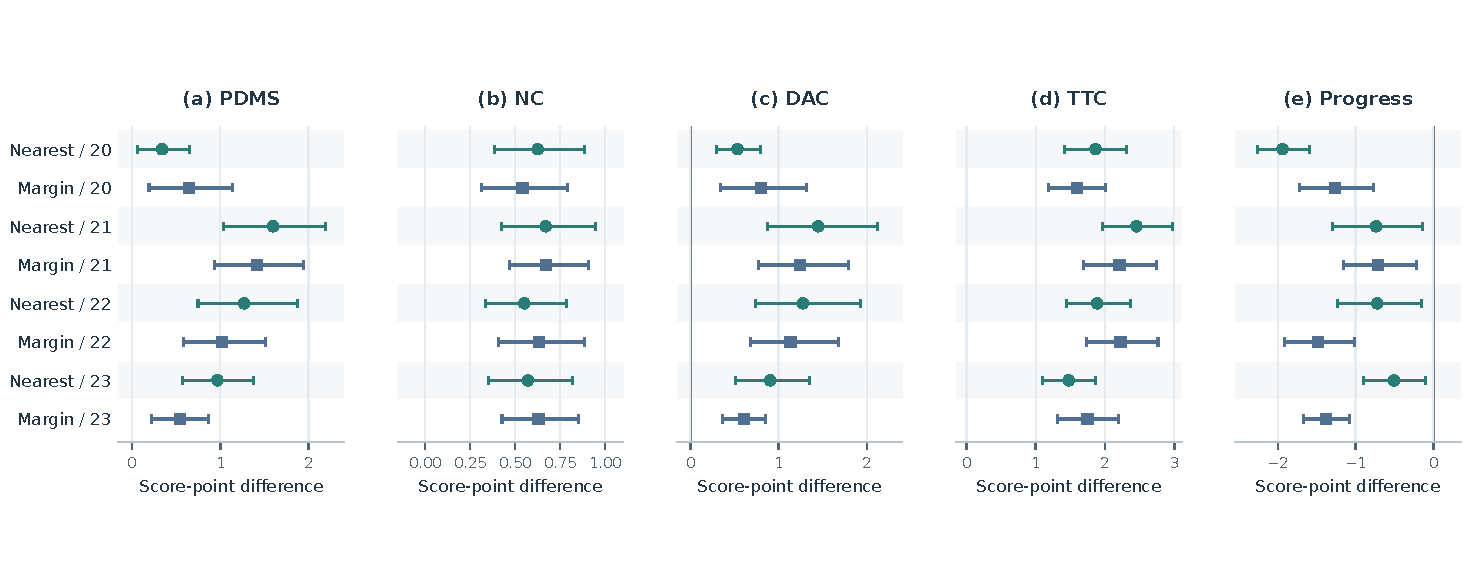
\includegraphics[width=0.9\textwidth]{figures/ral/fig3_target_contrasts.pdf}
\caption{\textbf{The target contrast repeats at four matched seeds.} Geometric minus PDMS targets, with conditional 95\% log-cluster intervals. Safety-component and total-score differences are positive; progress differences are negative. NC is a component score rather than a binary pass rate. Axis ranges differ. The contrasts share logs and reuse the PDMS policy within each seed.}
\label{fig:target_contrasts}
\end{figure*}

\subsection{Matched comparisons isolate the winner-rule effect}
Our primary comparison is between winner rules at the same training seed. Fig.~\ref{fig:target_contrasts} subtracts each PDMS-trained policy from its two geometric counterparts. \textbf{All eight contrasts favor geometric targets in PDMS, NC, DAC, and TTC, with paired 95\% log-cluster intervals above zero.} Total-score differences range from +0.340 to +1.598 points. Higher total scores accompany better safety-component scores despite lower progress in every comparison. The rule contrast is therefore more consistently resolved than the individual gains over SFT.



\subsection{Winner choice changes the fitted policy}\label{sec:winner}
Table~\ref{tab:training} compares all three winner rules against the matched SFT baseline. \textbf{All eight geometric runs repair more failures than they introduce in every safety component; all four PDMS runs show the reverse.} Fig.~\ref{fig:ledger} makes this distinction visible component by component. Net gate changes range from +171 to +279 for geometric targets and from $-330$ to $-125$ for PDMS targets.

\begin{table}[!t]
\centering\small
\caption{All 12 standard-budget policies on full navtest, relative to matched SFT (86.99). Brackets give 95\% log-cluster intervals; bold estimates have intervals above zero. Summary rows give mean $\pm$ sample SD across four seeds. Repairs and regressions appear in Fig.~\ref{fig:ledger}.}
\label{tab:training}
\setlength{\tabcolsep}{4pt}
\begin{tabular}{@{}llr@{}}\toprule
Winner & Seed & $\Delta$PDMS [95\% interval]\\\midrule
PDMS & 20 & +0.078 [$-0.473$,0.591]\\
PDMS & 21 & $-0.871$ [$-1.743$,$-0.043$]\\
PDMS & 22 & $-0.252$ [$-0.898$,0.336]\\
PDMS & 23 & $-0.149$ [$-0.751$,0.424]\\
Nearest & 20 & +0.418 [$-0.084$,0.912]\\
Nearest & 21 & \textbf{+0.73} [0.28,1.15]\\
Nearest & 22 & \textbf{+1.018} [0.755,1.274]\\
Nearest & 23 & \textbf{+0.820} [0.401,1.196]\\
Margin & 20 & \textbf{+0.72} [0.46,0.98]\\
Margin & 21 & +0.54 [$-0.04$,1.10]\\
Margin & 22 & \textbf{+0.763} [0.382,1.128]\\
Margin & 23 & +0.396 [$-0.204$,0.958]\\
\midrule
\multicolumn{3}{@{}l}{Across-seed summary ($n=4$ per rule)}\\
PDMS & Mean $\pm$ SD & $-0.299\pm0.406$\\
Nearest & Mean $\pm$ SD & $+0.747\pm0.250$\\
Margin & Mean $\pm$ SD & $+0.605\pm0.169$\\
\bottomrule
\end{tabular}
\end{table}

\begin{figure*}[!t]
\centering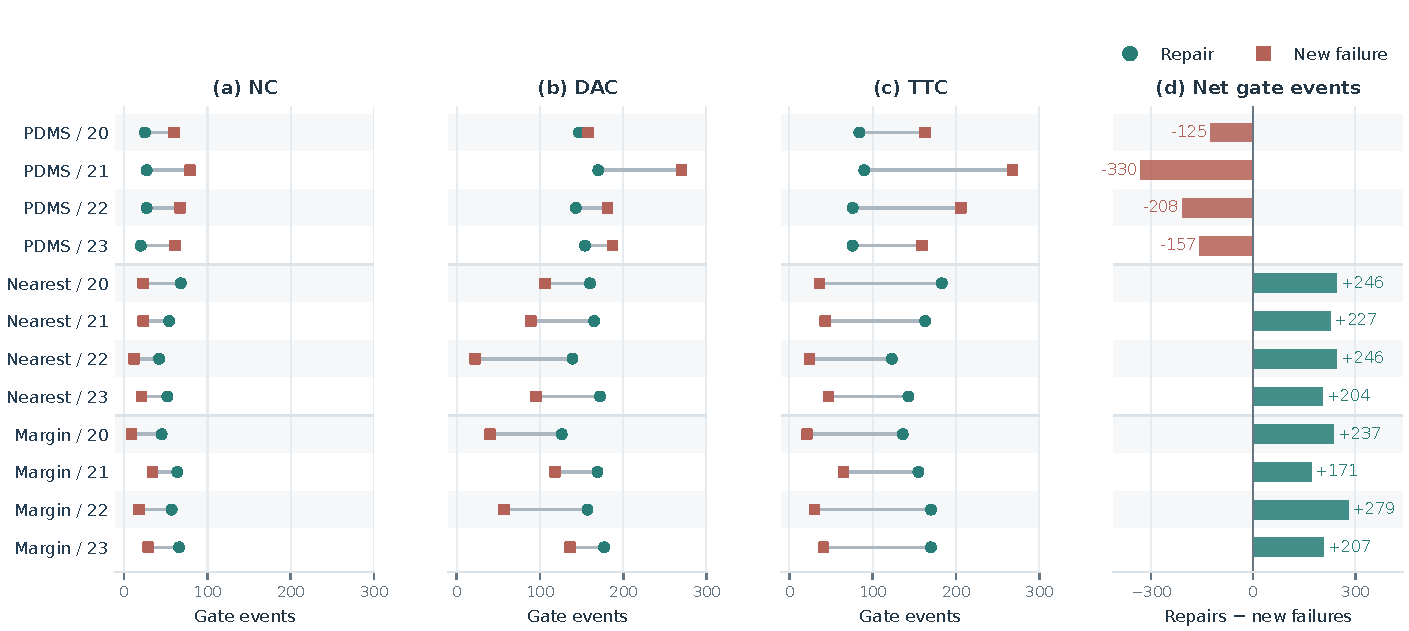
\includegraphics[width=0.8\textwidth]{figures/ral/fig2_repairs.pdf}
\caption{\textbf{Repairs must outweigh new failures.} Each row is one fitted policy evaluated against matched SFT. Teal marks repairs and rust marks newly failing scenes for each gate; the connecting line shows their balance. The right panel sums net events across gates. All four score-target policies have negative balances in every component, whereas all eight geometric-target policies have positive balances. Counts are descriptive; overlapping gate failures are counted separately.}
\label{fig:ledger}
\end{figure*}

Against SFT, all eight geometric runs have positive PDMS point estimates (+0.396 to +1.018), five with intervals above zero; the PDMS-trained runs range from $-0.871$ to +0.078. Every geometric point estimate exceeds every PDMS estimate, and the direct same-seed comparisons of Fig.~\ref{fig:target_contrasts} resolve the contrast.

Aggregate score alone understates the adverse changes in the score-based policies. PDMS seed 22 has an unresolved total-score change, $-0.252$ [$-0.898$,0.336], yet NC decreases by 0.288 [0.084,0.496] and TTC by 1.070 [0.631,1.531] while progress increases by 1.022 [0.420,1.574]. NC and TTC also decrease at the other three seeds, and progress increases at all four.

\subsection{Is geometric ranking necessary?}\label{sec:randwin}
To test whether explicit geometric ranking is needed to improve on score selection, we sample one winner uniformly from each eligible set. A fixed selection seed defines the target set, which is then used for three training seeds (20--22); loser construction, fitting recipe, and training scenes remain unchanged. These runs vary policy training, not the random target-set realization. \textbf{The random-winner policy outperforms the score-trained policy at every seed} (+0.46 [0.07, 0.84], +1.46 [1.02, 1.96], and +0.96 [0.67, 1.30] PDMS), and exceeds SFT by +0.54, +0.59, and +0.71. Table~\ref{tab:randwin} gives the three-seed means. Relative to nearest-reference and margin targets, the total-score difference is not resolved ($-0.11$ [$-0.29$, 0.05] and $-0.07$ [$-0.23$, 0.08]). The geometric rules retain small advantages in NC, DAC, and TTC, with intervals excluding zero, while the random-winner policy has higher progress.

\begin{table}[t]
\centering\small
\caption{Random eligible winner, seeds 20--22. All contrasts use the same three training seeds (20--22). Entries compare per-scene seed means (points; total with 95\% log-cluster interval conditional on the checkpoints).}
\label{tab:randwin}
\renewcommand{\arraystretch}{1.18}
\setlength{\tabcolsep}{3pt}
\begin{tabular}{@{}lrrrrr@{}}
\toprule
Contrast & Total & NC & DAC & TTC & EP \\
\midrule
Random $-$ SFT & \shortstack{+0.61\\{}[0.14, 1.04]} & +0.23 & +0.48 & +0.70 & +0.10 \\
Random $-$ PDMS & \shortstack{+0.96\\{}[0.63, 1.30]} & +0.53 & +0.88 & +1.76 & $-0.82$ \\
Random $-$ nearest & \shortstack{$-0.11$\\{}[$-0.29$, 0.05]} & $-0.09$ & $-0.20$ & $-0.31$ & +0.31 \\
Random $-$ margin & \shortstack{$-0.07$\\{}[$-0.23$, 0.08]} & $-0.09$ & $-0.18$ & $-0.25$ & +0.33 \\
\bottomrule
\end{tabular}
\end{table}

This control improves on score maximization without explicitly ranking candidates by geometry. The geometric rules retain safety-component advantages at lower progress, but their total-score advantages over random selection are unresolved; this is not an equivalence test. The result concerns one sampled target set and three training seeds, not arbitrary choices from the passing set. It does not identify the mediator of score selection's disadvantage. The progress-capped comparison below examines a possible explanation, but changes in training-scene support prevent attributing its outcome solely to progress preference.

\subsection{Restricting progress in score-based targets}\label{sec:capped}
The random control shows that geometric ranking is not required to improve on the score rule in these runs. We next test one feature of score-based selection: its preference for progress. Among passing candidates with equal comfort, score maximization retains a preference for greater evaluated progress (Section~\ref{sec:ordering}). We test a restricted version of this rule: select the highest-PDMS passing candidate whose progress does not exceed the mean reference progress. This cap restricts the allowable progress but still maximizes score within the restricted set. Loser construction, fitting recipe, and seeds remain unchanged. Scenes without a qualifying capped winner are omitted, reducing the training set from 988 to 860 pairs.

\textbf{All four capped policies have positive repair balances in every component} (Table~\ref{tab:capped}). Their mean PDMS change is $+0.425\pm0.358$ across seeds, with progress 0.21--1.10 points below SFT, and total-score gains over uncapped score training resolve at seeds 21--23. Their score gains remain below nearest-reference at seeds 20--22; the cap does not establish a uniformly preferable target rule. Because the cap also removes 128 training scenes and changes target displacement, the result is consistent with a role for progress preference but does not isolate it.

\begin{table}[t]
\centering\small
\caption{Progress-capped policies on full navtest. Score changes are relative to matched SFT or the same-seed uncapped PDMS policy; brackets give 95\% log-cluster intervals. Capped and uncapped training use 860 and 988 pairs, respectively. Net counts sum gate events.}
\label{tab:capped}
\setlength{\tabcolsep}{3pt}
\begin{tabular}{@{}crrr@{}}
\toprule
Seed & $\Delta$PDMS vs. SFT & Net events & $\Delta$PDMS vs. PDMS \\
\midrule
20 & $-0.024$ & \textbf{+146} & $-0.103$ [$-0.468$,0.237] \\
21 & +0.441 & \textbf{+268} & +1.312 [0.833,1.823] \\
22 & +0.432 & \textbf{+259} & +0.685 [0.253,1.156] \\
23 & +0.852 & \textbf{+274} & +1.001 [0.577,1.440] \\
\bottomrule
\end{tabular}
\end{table}

\subsection{Do target summaries explain the ordering?}\label{sec:targetstats}
Mean target statistics do not explain the rule ordering. PDMS and nearest targets have the same mean agent clearance (4.19\,m) and fraction below 2.5\,m (0.563), despite opposite repair balances. Margin targets have mean reference displacement near PDMS (0.385 versus 0.420\,m), yet positive repair balances.

For 300 shared training scenes, we pair each rule's target with base and seed-20 fitted outputs generated using the same scene-specific latent and ten-step deterministic integration. Targets need not share that latent. We measure $\hat\epsilon_w=\sqrt{\operatorname{mean}_s\|\widehat A-A^+\|^2}$ in normalized 24-dimensional relative-action space. Base-to-fitted errors are 0.246 to 0.245 (PDMS), 0.240 to 0.250 (margin), and 0.203 to 0.214 (nearest). Mean planar increment errors after undoing normalization are also similar for fitted margin and PDMS (0.116 and 0.123\,m); these are not integrated-waypoint position errors. These summaries do not explain the outcome contrast. Error tails and alignment with constraint boundaries remain unresolved, and applying Proposition~\ref{prop:margin} requires a compatible clearance and norm.

\section{Candidate Opportunity and Information}\label{sec:opportunity}
The training results concern how targets transfer into a policy. The following controls ask a different question: how much benefit can be extracted by selecting trajectories at inference, and what information enables that selection?
To assess candidate quality separately from policy fitting, we train a privileged histogram-based gradient-boosted tree (HGB) ranker on the 7,171-scene trainval candidate pool. It predicts scene-centered PDMS from 26 trajectory and 15 geometric features, derived from time-zero agents and drivable area, and selects among 16 navtest candidates without accessing their evaluation scores. We use 100 boosting iterations, learning rate 0.05, at most 31 leaves, $\ell_2$ regularization 1.0, and no early stopping. It measures the benefit of selection with additional information, not an equal-input alternative to the camera policy.

These controls use separate protocols, not additional matched training arms. The HGB ranker over 16 candidates gains 2.90 PDMS points [2.32,3.48] over independent SFT (oracle: +6.00), primarily through DAC repairs (377 repaired, 53 introduced). This test-time selection differs from the random-winner training control in Section~\ref{sec:randwin}. On DriveVLA-W0's Multi-Anchor variant, which generates and scores anchor-based trajectory candidates, ranking gains +1.09 [0.72,1.47] but repairs 175 TTC failures while introducing 298. Selection can thus raise score without preserving every safety component, and its privileged geometry means its gain is not what policy training must recover.

\section{Sensitivity to Sampling, Budget, and Scorer}

\subsection{Independent inference draws}
We first check whether the observed outcomes depend on
the random latents used to generate trajectories.
Three evaluations of the unchanged SFT policy produce
pairwise PDMS differences of $-0.002$, +0.045, and +0.047;
all 95\% log-cluster intervals include zero.

We then re-evaluate the three seed-20 policies using a new latent draw, comparing each with SFT under the same draw.
PDMS changes remain positive for nearest-reference
(+0.422 [$-0.117$,0.921]) and margin
(+0.777 [0.445,1.096]). The score-trained policy again
increases progress (+1.298) while reducing TTC
($-0.576$ [$-0.905$,$-0.241$]).
The main directions therefore repeat for these policies,
although not every total-score change is statistically
resolved. This check covers one training seed.

\subsection{Larger training budgets}
We also approximately double both the training-scene count
and the update budget. Margin and nearest-reference retain
positive PDMS gains over SFT: +0.774 [0.466,1.103] and
\textbf{+1.272 [0.913,1.628]}, respectively, with net gate
improvements of +292 and +333.

These runs show that the geometric rules retain their benefits at the larger tested budget. The extension covers only geometric rules at one seed each and changes data and updates jointly, so it is not a scaling trend.



\subsection{Winner-rule contrasts under NAVSIM v2 scoring}\label{sec:v2}
We re-score the saved trajectories of SFT, the twelve standard runs, and the four capped runs with the NAVSIM v2 one-stage scorer and its EPDMS aggregator~\cite{navsimv2}, under non-reactive traffic and under reactive traffic in which IDM agents respond to the ego trajectory. Each evaluation covers all 12,146 scenes without scoring errors; SFT scores 86.84 and 86.69, respectively. For each trained rule we average the four seeds' scores within each scene before computing paired differences and log-cluster intervals. This post hoc analysis reuses the same policies and scenes and is not closed-loop execution or the complete two-stage v2 benchmark.

\begin{table}[t]
\centering\small
\caption{Winner-rule comparisons under two v2 traffic settings. Entries are total-score differences between four-seed per-scene means, with 95\% log-cluster intervals conditional on the trained policies. }
\label{tab:v2}
\setlength{\tabcolsep}{3pt}
\begin{tabular}{@{}lcc@{}}
\toprule
Contrast & Non-reactive & Reactive (IDM) \\
\midrule
Margin $-$ PDMS & \textbf{+0.41} [0.04, 0.80] & \textbf{+0.59} [0.28, 0.96] \\
Nearest $-$ PDMS & \textbf{+0.51} [0.12, 0.95] & \textbf{+0.66} [0.30, 1.05] \\
Capped $-$ PDMS & +0.11 [$-0.20$, 0.46] & +0.27 [$-0.02$, 0.58] \\
PDMS $-$ SFT & $-0.30$ [$-0.95$, 0.29] & $-0.53$ [$-1.15$, 0.04] \\
\bottomrule
\end{tabular}
\end{table}

\textbf{The geometric-versus-score advantage persists in both traffic settings} (Table~\ref{tab:v2}). Non-reactive NC, DAC, TTC, and driving-direction advantages resolve for both geometric rules, as do reactive NC and TTC advantages; progress remains lower than under score-based training.

\textbf{Relative advantage does not establish improvement over SFT.} No rule has a resolved v2 total-score gain over SFT in either setting (reactive: +0.06 [$-0.37$,0.48] for margin and +0.13 [$-0.24$,0.51] for nearest). All four rules lose 0.55--0.67 lane-keeping points relative to SFT, and non-reactive PDMS training also reduces NC, TTC, and driving-direction compliance. These results support the relative winner contrast while exposing losses beyond the v1 verification gates.

\section{Discussion}
\subsection{Target quality is not training usefulness}
The score rule selects the best-scoring eligible candidate but produces worse policies than either geometric rule in the matched v1 comparisons. Random eligible targets also outperform score selection: explicit geometric ranking is not necessary for that improvement. Unresolved total-score differences do not establish equivalence, however; geometric rules retain safety-component advantages over random targets. Winner rules should therefore be validated through the policies they train, against both SFT and simple selection controls.

\subsection{Preservation and mechanism}
The ledger shows how regressions on common successes can outweigh repairs on rare failures. V2 further exposes lane-keeping losses outside the original verification gates, despite the geometric-versus-score advantage. Evaluation must therefore test preservation beyond the criteria used to qualify targets.

The gradient derivation locates winner dependence, and the margin bound states conditions for feasibility transfer; neither predicts the empirical ordering. Clearance, displacement, and fitting-error summaries do not explain the contrast. Error alignment with constraint boundaries remains a possible explanation. Capped targets also change scene support, precluding attribution to progress restriction alone. The controlled experiment identifies a winner-rule effect under the combined objective, not separate effects of preference loss, winner fitting, and expert anchoring.

\subsection{Scope of the evidence}
Training uses one frozen-backbone flow policy; Multi-Anchor only tests candidate ranking. Privileged ranking quantifies opportunity with extra information, not achievable camera-policy improvement. V2 re-scores saved trajectories rather than an observing, replanning policy. Four matched seeds (three for random winners) support repetition within this recipe; log-cluster intervals condition on these policies. The random control shares one target draw, and navtest was inspected during development. Generalization to other architectures, target draws, and closed-loop execution remains untested. These offline results motivate investigating target rankings in online RL but do not establish their effects under on-policy optimization.

\section{Conclusion}
Safety-qualified trajectories are not interchangeable as supervision. Under a fixed offline fitting recipe, changing the winner rule reverses the balance between repaired and newly introduced failures. Both geometric rules and a random-eligible control improve on score-maximizing targets in the tested v1 comparisons; explicit geometric ranking is therefore not necessary for this improvement. Geometric rules retain component-wise advantages over random targets.
The broader finding concerns how supervision should be evaluated: through the behavior of the fitted policy, not only the quality of its targets. V2 re-scoring reinforces this distinction by retaining the geometric-versus-score advantage while exposing lane-keeping losses. Repairs, regressions, and behavior beyond the verification gates together determine whether post-training preserves existing successes while improving failures.

\begin{thebibliography}{99}
\bibitem{sweetspot}
Y. Xiao et al., ``Finding the sweet spot: Preference data construction for scaling preference optimization,'' in \emph{Proc. 63rd Annu. Meeting Assoc. Comput. Linguistics (ACL)}, 2025, pp. 12538--12552.

\bibitem{whatmatters}
Y. Pan, Z. Cai, H. Zhong, G. Chen, and C. Wang, ``What matters in data for DPO?'' in \emph{Adv. Neural Inf. Process. Syst. (NeurIPS)}, vol. 38, 2026, pp. 44689--44716.

\bibitem{correctanswers}
X. Tian et al., ``Not all correct answers are equal: Why your distillation source matters,'' arXiv:2505.14464, 2025.

\bibitem{drivevla}
Y. Li et al., ``DriveVLA-W0: World models amplify data scaling law in autonomous driving,'' in \emph{Proc. Int. Conf. Learn. Represent. (ICLR)}, 2026.

\bibitem{diffpolicy}
C. Chi et al., ``Diffusion policy: Visuomotor policy learning via action diffusion,'' \emph{Int. J. Robot. Res.}, vol. 44, no. 10--11, pp. 1684--1704, 2025.

\bibitem{pi0}
K. Black et al., ``$\pi_0$: A vision-language-action flow model for general robot control,'' arXiv:2410.24164, 2024.

\bibitem{diffdrive}
B. Liao et al., ``DiffusionDrive: Truncated diffusion model for end-to-end autonomous driving,'' in \emph{Proc. IEEE/CVF Conf. Comput. Vis. Pattern Recognit. (CVPR)}, 2025, pp. 12037--12047.

\bibitem{diffdrivev2}
J. Zou et al., ``DiffusionDriveV2: Reinforcement learning-constrained truncated diffusion modeling in end-to-end autonomous driving,'' arXiv:2512.07745, 2025.

\bibitem{takead}
D. Liu et al., ``TakeAD: Preference-based post-optimization for end-to-end autonomous driving with expert takeover data,'' \emph{IEEE Robot. Autom. Lett.}, vol. 11, no. 2, pp. 1738--1745, 2025.

\bibitem{dpo}
R. Rafailov, A. Sharma, E. Mitchell, C. D. Manning, S. Ermon, and C. Finn, ``Direct preference optimization: Your language model is secretly a reward model,'' in \emph{Adv. Neural Inf. Process. Syst. (NeurIPS)}, vol. 36, 2023, pp. 53728--53741.

\bibitem{diffdpo}
B. Wallace et al., ``Diffusion model alignment using direct preference optimization,'' in \emph{Proc. IEEE/CVF Conf. Comput. Vis. Pattern Recognit. (CVPR)}, 2024, pp. 8228--8238.

\bibitem{awr}
X. B. Peng, A. Kumar, G. Zhang, and S. Levine, ``Advantage-weighted regression: Simple and scalable off-policy reinforcement learning,'' arXiv:1910.00177, 2019.

\bibitem{bond}
P. G. Sessa et al., ``BOND: Aligning LLMs with best-of-N distillation,'' in \emph{Proc. Int. Conf. Learn. Represent. (ICLR)}, 2025, pp. 59040--59060.

\bibitem{dppo}
A. Ren et al., ``Diffusion policy policy optimization,'' in \emph{Proc. Int. Conf. Learn. Represent. (ICLR)}, 2025.

\bibitem{flowmatching}
Y. Lipman, R. T. Q. Chen, H. Ben-Hamu, M. Nickel, and M. Le, ``Flow matching for generative modeling,'' arXiv:2210.02747, 2022.

\bibitem{drivereferee}
F. Yu et al., ``DriveReferee: Geometric safety verdicts need not be learned for driving world-action models,'' arXiv:2609.22762, 2026.

\bibitem{cpo}
J. Achiam, D. Held, A. Tamar, and P. Abbeel, ``Constrained policy optimization,'' in \emph{Proc. Int. Conf. Mach. Learn. (ICML)}, 2017, pp. 22--31.

\bibitem{shielding}
M. Alshiekh et al., ``Safe reinforcement learning via shielding,'' in \emph{Proc. AAAI Conf. Artif. Intell.}, 2018.

\bibitem{dagger}
S. Ross, G. Gordon, and D. Bagnell, ``A reduction of imitation learning and structured prediction to no-regret online learning,'' in \emph{Proc. Int. Conf. Artif. Intell. Statist. (AISTATS)}, 2011, pp. 627--635.

\bibitem{navsim}
D. Dauner et al., ``NAVSIM: Data-driven non-reactive autonomous vehicle simulation and benchmarking,'' in \emph{Adv. Neural Inf. Process. Syst. (NeurIPS), Datasets and Benchmarks Track}, 2024.

\bibitem{navsimv2}
W. Cao et al., ``Pseudo-simulation for autonomous driving,'' in \emph{Proc. Conf. Robot Learn. (CoRL)}, 2025.

\end{thebibliography}
\end{document}
